
\documentclass{svproc}
\usepackage[T2A]{fontenc}
\usepackage[utf8]{inputenc}
\usepackage[english,russian]{babel}
\usepackage{graphicx}
\graphicspath{ {img/} }
%
% RECOMMENDED %%%%%%%%%%%%%%%%%%%%%%%%%%%%%%%%%%%%%%%%%%%%%%%%%%%
%

% to typeset URLs, URIs, and DOIs
\usepackage{url}
\def\UrlFont{\rmfamily}

\begin{document}
\mainmatter              % start of a contribution
%
\title{Краткий обзор на научные статьи}
%
\author{Сажникова О.В.}
%
\authorrunning{Сажникова О.В.} % abbreviated author list (for running head)
%
%%%% list of authors for the TOC (use if author list has to be modified)
\tocauthor{Сажникова Ольга Владимировна}
%
\institute{Ульяновский Технический Университет, г. Ульяновск, Россия}
\maketitle              % typeset the title of the contribution

\begin{abstract}
В данной статье рассматривается краткий обзор на 5 рускоязычные и 5 англоязычные статьи в области применения нейронных сетей в распознавании паталогий на рентегеновских снимках легких человека.
% 
\keywords{нейронные сети, сверточные нейронные сети, обработка изображений}
\end{abstract}
%
В настоящее время сфера информационных технологий очень активно развивается и тесно контактирует с другими сферами жизнедеятельности человека, в том числе и с медециной. Например, для диагностики различных паталогий в легких человека, необходимо сделать рентгеновский снимок, глядя на который врач ставит диагноз. Но из-за некомпетентности или невнимательности врач может поставить неверный диагноз, который сильно навредит здоровью человека. Для автоматизации и улучшения качества постановки диагноза сфера информационных технологий предлагает к использованию сверточные нейронные сети, которые взяв в качестве входных данных рентгеновский снимок, на выходе выдадут крайне точный диагноз.

\section{Русскоязычные статьи}
%
В первой статье происходит знакомство с самой нейронной сетью, сравнение нейронной сети с биологическими нейроннами. Нейронная сеть – это математическая модель, которая может быть представлена в виде программы или программно-аппаратного обеспечения. Она создана по принципу работы биологических нейронных сетей млекопитающих и образует систему взаимодействующих между собой искусственных нейронов. [1] На вход нейрону поступают входные данные x. Входы между нейроннами соединены синаптической связью S, у которой есть свой вес w, который определяет, как соответствующий вход нейрона влияет на его состояние. Таким образом состояние нейрона записывается как: 
\begin{equation}
  S = \sum\limits_{i=1}^n x_{i} w_{i}\ ,
\end{equation}


Во второй статье рассматривается применение каждой группы сверточной нейронной сети. В основном сверточные нейронные сети решают задачи задачу обнаружения и классификации объектов. 

Нейросетевые архитектуры для обнаружения и распознавания объектов можно разделить на две большие группы:

1. Архитектуры, обрабатывающие регионы на изображении (R-CNN).

2. Архитектуры, обрабатывающие поступившее изображение целиком (YOLO, SSD). [2]

YOLO: Архитектура YOLO изначально разрабатывалась для задач реального времени. В алгоритме YOLO изображение разделяется на ячейки с использованием сетки. Для каждой ячейки сетки оценивается
вероятность присутствия объекта вообще, затем строятся несколько наиболее вероятных положений объекта в виде прямоугольников с центром в данной ячейке, после чего для каждого полученного прямоугольника выполняется оценка вероятностей наличия в нем объектов каждого рассматриваемого класса.

Для решения задачи обнаружения объектов Faster R-CNN в настоящее время является одной из часто используемых архитектур на основе глубокого обучения.

Работа R-CNN состоит из трех основных этапов:

1. Исходное изображение разбивается на регионы, в
которых могут находиться объекты. С этой целью применяется алгоритм Selective Search, генерирующий
2000 различных областей, которые с наибольшей вероятностью содержат объекты.

2. Каждый регион подается на вход соответствующей обученной сверточной нейронной сети, которая
извлекает вектор признаков для своего региона.

3. Вектора признаков подаются на вход набора SVM,
выполняющих функцию классификации. Каждая SVM
обучена для определения одного класса объектов. Кроме
того, для уточнения параметров охватывающего объект
прямоугольника применяется линейная регрессия.

Архитектура SSD обеспечивает значительный
прирост скорости обработки по сравнению с Faster
R-CNN.

Работу SSD можно
описать следующим образом:

1. Исходное изображение проходит через ряд сверточных слоев, что в результате дает набор карт признаков для
разных масштабов (например, 19×19, 10×10, 5×5 и т.д.).

2. В каждой точке каждой карты признаков применяется сверточный фильтр размера 3×3 для получения
множества описывающих прямоугольников.

3. Для каждого прямоугольника одновременно оцениваются пространственное смещение и вероятность
нахождения объекта.

4. В процессе обучения истинные описывающие
объект прямоугольники сопоставляются с предсказанными для исключения ложных обнаружений

В третьей статье рассказывается об особенностях сверточных нейронных сетей при обработке изображений. Для лучшей работы нейронной сети перед началом работа с изображением проводят некоторые работы. К изображениям необходимо применять искажающие преобразования: операции
масштабирования, обрезание границ изображения с последующим приведением его к
заданному размеру с билинейной интерполяцией, а также эрозии и дилатации случайных
прямоугольных областей всего изображения. [3]

В четвертой статье раскрывается структура сверточной нейронной сети и то, как обучать сеть. Наглядная структура сверточной нейронной сети представлена на рис.1.

\begin{figure}[h]
    \centering
    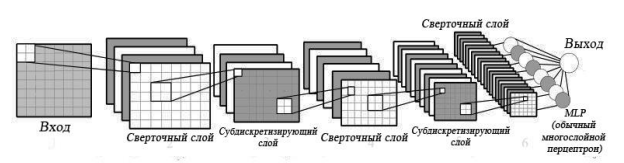
\includegraphics[width=0.90\textwidth]{picture_1}
    \caption{Структура сверточной нейронной сети}
    \label{fig:picture_1}
\end{figure}

Одним из подходов обучения сверточных
нейронных сетей является обучение с нуля. [4] На практике метод полного обучения сети реализуется крайне редко, так как проблематично
найти набор данных достаточного размера для обучения сети. Вместо этого обычно принято брать
уже обученную сверточную нейронную сеть и использовать ее для решения поставленной задачи.

В пятой статье рассматривается применение сверточной нейронной сети для анализа рентгеновских снимков легких человека. Чаще всего паталогией явяется некая область, которая проявляется как затемнение легочного поля в виде очаговой тени. [5] Примерный алгоритм обнаружения паталогии на снимке представлен на рис.2

\begin{figure}[h]
    \centering
    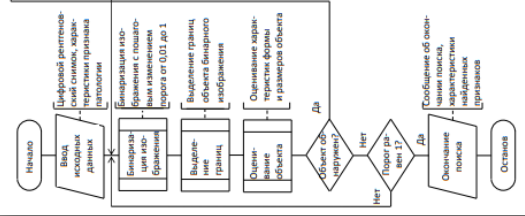
\includegraphics[width=0.90\textwidth]{picture_2}
    \caption{Алгоритм обнаружения паталогии}
    \label{fig:picture_2}
\end{figure}

\section{Англоязычные статьи}
%
В шестой статье рассматривается работа нейронной сети, и объясняется разница между Convolutional Neural Network (CNN) и Recurrent Neural Network (RNN). В глубоком обучении сверточные нейронные сети (CNN) представляют собой класс ANN с прямой связью, которые эффективно применяются в компьютерном зрении. Рекуррентные нейронные сети (RNN) - это еще один тип нейронных сетей, который используется для решения сложных задач машинного обучения, включающих последовательности входных данных. [6] Авторы статьи провели экспериментальные замеры распознавания сорняков среди других растений используя данные 2 сети. Результат показал, что RNN в сочетании с LSTM подходит для обнаружения сорняков среди других методов, но CNN всегда на первом месте с точки зрения скорости и точности. 

В седьмой статье подробнее рассматривается алгоритм работы сверточной нейронной сети. В рамках классического подхода архитектура CNN описывается следующими параметрами: 

N - размерность плоскости в слое; для входного слоя плоскость представляет собой произведение высоты H и ширины W изображения;

D - глубина входного слоя; в нашем случае - количество цветовых каналов в изображении; 

P - количество строк и столбцов, добавленных к границам слоя, предшествующего слою свертки, и заполненных нулями; 

S - смещение между фильтрами, на которых генерируются сигналы нейронов в слоях свертки и субдискретизации; 

F - размер квадратных фильтров слоя свертки; 

Filters - глубина слоя свертки (количество фильтров); 

U - размер квадратного окна в слое слияния; 

Subf - тип функции, описывающей слой подвыборки (max - максимальная или avg - средняя оценка); 

K - количество нейронов в полностью связанном слое; 

C - количество классов в задаче; классификатор определяет, к какому классу относится данный объект (в нашей классификации C=2, т.е. полип/не полип); [7]
AF - функция активации нейрона: пороговая функция (2), сигмоидная функция (3) или функция гиперболического тангенса (4):

\begin{equation}
  y = {\rm Max\,} \left\{0,1\right\}\ ,
\end{equation}
\begin{equation}
  y = 1/[1+e^{-x}]\ ,
\end{equation}
\begin{equation}
  y = \tan{x}\ ,
\end{equation}

И представляется на рис.3

\begin{figure}[h]
    \centering
    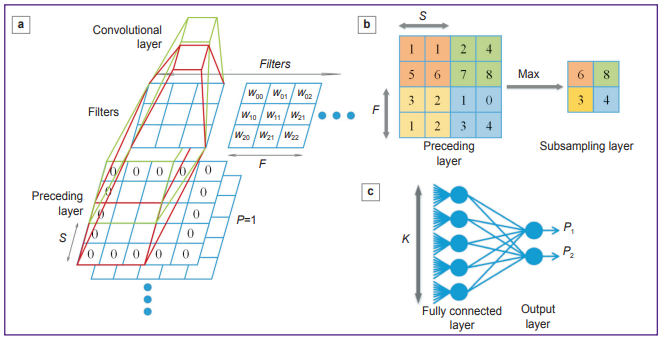
\includegraphics[width=0.90\textwidth]{picture_3}
    \caption{Архитектура CNN}
    \label{fig:picture_3}
\end{figure}

В восьмой статье рассматривается вопрос повышения эффективности работы обычной нейронной сети, что привело к появлению сверточной нейронной сети. Предполагается, что все пиксели изображения можно привязать к одному нейрону, но этот вариант ограничен тем, что в результате получается большое количество весов, что приведет к длительному времени вычисления суммы каждого нейрона. Также этот метод будет неустойчив к переобучению, поэтому нейронная сеть будет неэффективно работать с примерами, которые не являются частью обучающего множества. [8] Для решения этих проблем была разработана архитектура, в которой каждый нейрон связан только с небольшой областью изображения, а все нейроны имеют одинаковые веса. Этот процесс представляет собой свертку изображения и отображен на рис.4.

\begin{figure}[h]
    \centering
    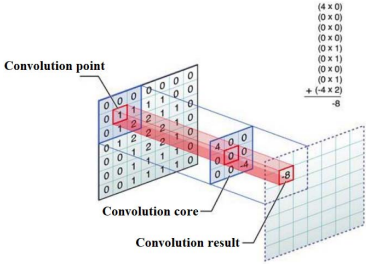
\includegraphics[width=0.70\textwidth]{picture_4}
    \caption{Свертка изображения}
    \label{fig:picture_4}
\end{figure}

В девятой статье рассматривается применение сверточной нейронной сети для обработки звуков: определение эмоционального состояния. Для анализа эмоционального состояния человека обычно используются следующие биосигналы: гальваническая реакция кожи (GSR), электромиограмма (EMG), частота сердечных сокращений (HR), частота дыхания (RR) и электроэнцефалограмма (EEG). Из них ЭЭГ наиболее интересна; она отражает активность коры головного мозга, которая формирует ряд эмоциональных реакций. [9] На всех этапах эксперимента, включая запись и обработку сигнала, а также обучение модели, использовался Python и библиотеки scikit-learn и Keras.

В десятой статье рассматривается применение сверточной нейронной сети для распознавания образов людей без медицинской маски. Авторы статьи рассматривают проблему сети обратного распространения. Разработчики сети ResNet (остаточная сеть) заметили, что с увеличением количества слоев сверточная нейронная сеть может начать деградировать. Эта проблема обучения называется проблемой исчезающего градиента. Суть проблемы заключается в том, что при работе с методом обратного распространения используется правило цепочки. Если градиент имеет небольшое значение в конце сети, то к моменту достижения начала сети он может принять бесконечно малое значение. Это может привести к невозможности обучения сети. [10] В ResNet предполагалось, что если CNN достигла предела точности на определенном слое, то все последующие слои должны выродиться в идентичное преобразование, но этого не происходит из-за сложности обучения глубоких сетей. В результате исследований ResNet было предложено ввести блок остатков. При его использовании входные данные передаются по короткому пути, минуя слои преобразования, и добавляются к результату (рис. 5).

\begin{figure}[h]
    \centering
    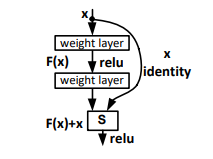
\includegraphics[width=0.50\textwidth]{picture_5}
    \caption{Идея ResNet}
    \label{fig:picture_5}
\end{figure}

Это дало толчок для создания архитектуры VGG-16. Число 16 в названии VGG-16 относится к тому, что она имеет 16 слоев, которые имеют определенные веса. Преимуществом VGG-16 является простота реализации. Одним из недостатков VGG-16 была низкая скорость обучения. В настоящее время, благодаря развитию компьютерных технологий, этот недостаток устранен. Эта архитектура хорошо документирована и используется для выполнения задач классификации средней сложности. Набор данных для обучения VGG-16 не обязательно должен быть большим.


%
% ---- Bibliography ----
%
\begin{thebibliography}{6}
%

\bibitem {krasn}
Краснова А. Ю.: ИЗУЧЕНИЕ ПРИНЦИПА РАБОТЫ СВЕРТОЧНОЙ НЕЙРОННОЙ СЕТИ.
ИМиМ КФУ (Институт математики и механики им. Лобачевского
Казанского Федерального Университета), Россия, Казань (2020).

\bibitem {eroh:ersh}
Ерохин Д.Ю., Ершов М.Д.: СОВРЕМЕННЫЕ СВЕРТОЧНЫЕ НЕЙРОННЫЕ СЕТИ ДЛЯ ОБНАРУЖЕНИЯ И РАСПОЗНАВАНИЯ ОБЪЕКТОВ: ЦИФРОВАЯ ОБРАБОТКА СИГНАЛОВ (2018).

\bibitem {pchel:arzam}
Пчелинцев С.Ю., Арзамасцев А.А.: ОСОБЕННОСТИ ИСПОЛЬЗОВАНИЯ СВЕРТОЧНЫХ НЕЙРОННЫХ СЕТЕЙ ДЛЯ АНАЛИЗА ИЗОБРАЖЕНИЙ В ВИДЕОПОТОКЕ: 	МАТЕРИАЛЫ И МЕТОДЫ ИННОВАЦИОННЫХ ИССЛЕДОВАНИЙ И РАЗРАБОТОК, Уфа (2018).

\bibitem {alex}
Алексеенко Ю.В.: РАЗРАБОТКА СИСТЕМЫ РАСПОЗНАВАНИЯ ИЗОБРАЖЕНИЙ НА ОСНОВЕ СВЕРТОЧНЫХ НЕЙРОННЫХ СЕТЕЙ: "ТЕХНИЧЕСКИЕ НАУКИ" Институт сферы обслуживания и предпринимательства (филиал) ДГТУ, г. Шахты
Morgan Kaufmann, San Francisco (2017)

\bibitem {fand:koles}
 Фандеев В.П., Колеснов Д.В.: ИНФОРМАЦИОННАЯ ТЕХНОЛОГИЯ ПОИСКА ПРИЗНАКОВ ПАТОЛОГИИ НА РЕНТГЕНОВСКОМ СНИМКЕ ЛЕГКИХ: Медицина и здравоохранение (2018)

\bibitem {fand:koles}
 S.V. Aksenov, K.A. Kostin, A.V. Ivanova, J. Liang, A.V. Zamyatin: An Ensemble of Convolutional Neural Networks for the Use in Video Endoscopy: Advanced Researches (2017)
 
 \bibitem {fand:koles}
 D. Y. Manylov: CURRENT DIRECTIONS IN THE DEVELOPMENT OF NEURAL NETWORKS: Reshetnev Siberian State University of Science and Technology (2019)
 
 \bibitem {fand:koles}
 Savinov V.B., Botman S.A., Sapunov V.V., Petrov V.A., Samusev I.G., Shusharina N.N.: ELECTROENCEPHALOGRAM-BASED EMOTION RECOGNITION USING A CONVOLUTIONAL NEURAL NETWORK: ORIGINAL RESEARCH NEUROPHYSIOLOGY (2019)
 
 \bibitem {fand:koles}
 O. I. Sheremet, O. Ye. Korobov, O. V. Sadovoi, Yu. V. Sokhina
: INTELLIGENT SYSTEM BASED ON A CONVOLUTIONAL NEURAL NETWORK
FOR IDENTIFYING PEOPLE WITHOUT BREATHING MASKS: Applied Aspects of Information Technology (2020)

\bibitem {fand:koles}
Brahim Jabir, Loubna Rabhi, Noureddine Falih: RNN- and CNN-based weed detection for crop improvement: An overview: Foods and Raw Materials (2021)


\end{thebibliography}
\end{document}
